% ****** Start of file apssamp.tex ******
%
%   This file is part of the APS files in the REVTeX 4.1 distribution.
%   Version 4.1r of REVTeX, August 2010
%
%   Copyright (c) 2009, 2010 The American Physical Society.
%
%   See the REVTeX 4 README file for restrictions and more information.
%
% TeX'ing this file requires that you have AMS-LaTeX 2.0 installed
% as well as the rest of the prerequisites for REVTeX 4.1
%
% See the REVTeX 4 README file
% It also requires running BibTeX. The commands are as follows:
%
%  1)  latex apssamp.tex
%  2)  bibtex apssamp
%  3)  latex apssamp.tex
%  4)  latex apssamp.tex
%
\documentclass[%
 reprint,
%superscriptaddress,
%groupedaddress,
%unsortedaddress,
%runinaddress,
%frontmatterverbose, 
%preprint,
%showpacs,preprintnumbers,
%nofootinbib,
%nobibnotes,
%bibnotes,
 amsmath,amssymb,
 aps,
%pra,
%prb,
%rmp,
%prstab,
%prstper,
%floatfix,
]{revtex4-1}

\usepackage{graphicx}% Include figure files
\usepackage{dcolumn}% Align table columns on decimal point
\usepackage[spanish]{babel}
\selectlanguage{spanish} 
\usepackage[utf8]{inputenc}
\usepackage{bm}% bold math
%\usepackage{hyperref}% add hypertext capabilities
%\usepackage[mathlines]{lineno}% Enable numbering of text and display math
%\linenumbers\relax % Commence numbering lines
\usepackage{float}
%\usepackage[showframe,%Uncomment any one of the following lines to test 
%%scale=0.7, marginratio={1:1, 2:3}, ignoreall,% default settings
%%text={7in,10in},centering,
%%margin=1.5in,
%%total={6.5in,8.75in}, top=1.2in, left=0.9in, includefoot,
%%height=10in,a5paper,hmargin={3cm,0.8in},
%]{geometry}
\usepackage[font=footnotesize,labelfont=bf]{caption}
\usepackage{hyperref}
\newcommand{\subtitle}[1]{%
\posttitle{%
    \par\end{center}
\begin{center}\large#1\end{center}
\vskip0.5em}%
}
\begin{document}

%\preprint{APS/123-QED}

\title{Doble Rendija\\ \textit{Estudio de la dualidad de onda partícula} }% Force line breaks with \\

%\subtitle{Estudio de la dualidad de onda partícula}

\author{Jose Alejandro Montaña Cortés}
\email{ja.montana@uniandes.edu.co}
% \altaffiliation[Also at ]{Departamento de Física, Universidad de los Andes}
\author{Jesús David Rincón Puche}%
\email{jd.rincon883@uniandes.edu.co}
\affiliation{Departamento de Física, Universidad de los Andes}%

%\collaboration{}%\noaffiliation

\date{\today}% It is always \today, today,
             %  but any date may be explicitly specified

\begin{abstract}

El experimento de la doble rendija es un experimento que tiene mucha importancia en la física, porque muestra la dualidad onda-partícula de la luz. En esta práctica se realizaron dos experimentos: En el primero se utiliza un láser para encontrar el patrón de interferencia que este posee, de manera cualitativa y cuantitativa, para confirmar los cálculos analíticos al considerar el campo eléctrico como una onda monocromática, propiedad que también presenta el láser. Se observó con éxito como el láser sigue el patrón esperado en la difracción tanto para una rendida, como para la doble rendija y se encuentra una discrepancia del 23\% en lo esperado, atribuido posiblemente al rango de distancia que los máximos de las rendijas poseen. En el segundo experimento usamos luz blanca y un filtro de luz verde, para hacer un conteo de fotones que pasan por un detector. Al comparar los tiempos de viaje de un solo fotón y el tiempo de detección del contador, se encontró la naturaleza corpuscular de la luz.

\end{abstract}
\maketitle
%\tableofcontents

%---------------------INTRODUCCIÓN------------------
\section{Introducción}
Desde mediados de 1600 hasta inicios de 1900 se discutió si la luz debía ser considerada como una onda o como una partícula. Tal discusión se originó cuando el científico holandés C.Huygens conoce a  I. Newton en 1689, en esta fecha, Huygens publica su  teoría ondulatoria de la luz. Por otra parte, Newton opta por describir la naturaleza de la luz por medio de lo que él llamó “corpúsculos”. No obstante, con los desarrollos posteriores de Fresnel y Maxwell se ratificaba el comportamiento de tipo ondulatorio en la luz, con lo cual a finales de 1800 se creía que esta “dualidad” en la teoría parecía haberse esclarecido. Sin embargo, con el descubrimiento del efecto Compton y el efecto fotoeléctrico la descripción de la luz como cuantos de luz o como “corpúsculos” volvió a tomar fuerza. Posteriormente gracias al desarrollo de la mecánica cuántica el concepto de tomar a una partícula como un objeto que además exhibe propiedades de onda fue bien acogida por la comunidad científica y esta tomó bastante fuerza a mediados de 1900. En este experimento se estudiará las propiedades de onda y partícula que posee la luz al efectuar un montaje similar al propuesto por Young en 1803 en donde se hace pasar un haz de luz por medio de una doble rendija y así hacer uso de la teoría de difracción e interferencia de la óptica clásica para explicar el fenómeno. Posterior a esto con el fin de observar el comportamiento de partícula se envía una cantidad “pequeña” de fotones para que pase por una de las rendijas en un momento dado, esto con el fin de mostrar la dualidad de onda partícula de la luz.
\section{Desarrollo teórico}
\begin{figure}[ht]
\center{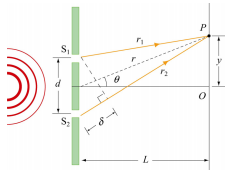
\includegraphics[width=0.4\textwidth]
{../Figuras/double_rendija.PNG}}
\caption{\label{doble rendija} Diagrama geométrico de la luz pasando por la doble rendija, de acá se puede deducir que $\delta=r_2-r_1\approx d\sin(\theta)$, lo cual es valido si la razón entre distancia entre las rendijas y la distnacia al detector es pequeña ($d/L\ll 1$)   (tomado de \cite{MIT}).}
\end{figure}

Gracias al desarrollo de la electrodinámica, se logró entender el comportamiento de la luz por medio de una ondas electromagnéticas. Debido a esto, la intensidad de la luz proveniente de 2 fuentes distintas\footnote{Para nuestro caso 2 rendijas}, puede escribirse como:
\[I(z,t)=\vec{E}(z,t)\cdot \vec{E}(z,t),\]
pero dado que $I(z,t)$ varia muy rápido en el tiempo, se toma el promedio de esta cantidad sobre un tiempo $T'$ grande, múltiplo del periodo $T$, con lo cual se tiene entonces que:
\[I(z)\propto\ \frac{1}{T'}\int_{0}^{T'}\vec{E}(z,t)\cdot \vec{E}(z,t) dt \sim \langle \vec{E}\cdot \vec{E}\rangle.\]
Dado que acá $\vec{E}$ representa el campo total y este a su vez está conformado por la suma de dos campos (uno de cada fuente), se tiene entonces que la intensidad está dada por,
\begin{equation*}
  \langle \vec{E}\cdot \vec{E}\rangle = \langle (\vec{E_1}+\vec{E_2})\cdot (\vec{E_1}+\vec{E_2})\rangle,
\end{equation*}
\begin{equation}
I\sim \langle E_1^2\rangle+\langle E_2^2\rangle+2\langle \vec{E_1}\cdot  \vec{E_2}\rangle,
\label{difrac}
\end{equation}
donde el térmico cruzado $\langle \vec{E_1}\cdot  \vec{E_2}\rangle$ es el que origina la interferencia. Con el fin de determinar una función para $I$ que contenga valores fácilmente medibles en el laboratorio, es posible escribir $\vec{E_1}$ y $\vec{E_2}$ en términos de ondas monocromáticas y coherentes.
\begin{align}
\vec{E_1}&=\vec{E_0}\sin(\omega t)   &  \vec{E_2}&=\vec{E_0}\sin(\omega t+ \phi),
\label{campos electricos}
\end{align}
con lo que efectuando la integral y reescribiendo el producto de los  se tiene entonces que \footnote{En donde se efectuó la integral
\[ \frac{1}{T}\int_{0}^{T}\sin^2\left(\omega t+\frac{\phi}{2}\right)=\frac{1}{2}\]
}
\begin{multline}
I\sim  \langle \vec{E}\cdot \vec{E}\rangle = 4E_0^2 \cos^2\left(\frac{\phi}{2}\right)\langle\sin^2\left(\omega t+\frac{\phi}{2}\right)\rangle \\
=2E_0^2\cos^2\left(\frac{\phi}{2}\right).
\label{intensidad_1}
\end{multline}
Con esto se tiene entonces que para que haya interferencia de tipo constructiva, es necesario que $\phi=2\pi$, lo cual corresponde a una diferencia de camino de $\delta=\lambda$, donde $\lambda$ corresponde la longitud de onda de la luz y $\delta$ es la diferencia de caminos entre los dos campos eléctricos. Así de esta forma se deduce que
\begin{equation}
\phi = \frac{2\pi d}{\lambda}\sin\theta,
\label{relacion_fase}
\end{equation}
sustituyendo \eqref{relacion_fase} en \eqref{intensidad_1} se tiene que
\begin{equation}
I=I_0\cos^2\left(\frac{\pi d \sin\theta}{\lambda}\right).
\label{interferencia}
\end{equation}
De una forma similar, se puede mostrar que para una sola rendija la intensidad  de la luz está dada por
\begin{equation}
I=I_0\left(\frac{\sin\alpha}{\alpha}\right)^2,
\label{difraccion}
\end{equation}
en donde
\begin{equation}
\alpha=\frac{\pi a}{\lambda}\sin\theta,
\end{equation}
\begin{figure}[h]
\center{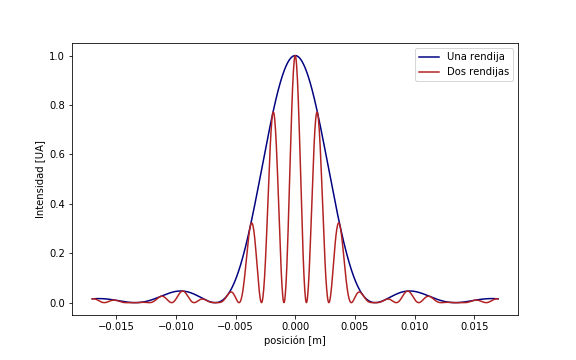
\includegraphics[width=0.4\textwidth,trim={1.5cm 1cm 1.5cm 0}]
{../Figuras/Ejemplo_interferencia.png}}
\caption{\label{ejemplo interferencia} Ejemplo de la intensidad predicha por la ecuación \eqref{Intensidad_total} para el caso de las 2 rendijas (roja) y \eqref{difraccion} para el caso de una rendija (azul).}
\end{figure}
con $a$ la longitud de la rendija por la que pasa la luz. Por ultimo se tiene que la intensidad del patrón de luz debido a la difracción y la interferencia es el producto de las ecuaciones \eqref{interferencia} y \eqref{difraccion}
\begin{equation}
I=I_0\left(\frac{\sin\alpha}{\alpha}\right)^2\cos^2\left(\frac{\pi d \sin\theta}{\lambda}\right).
\label{Intensidad_total}
\end{equation}
Las ecuaciones \eqref{Intensidad_total} y \eqref{difraccion} se muestran en la figura \ref{ejemplo interferencia}, ambas gráficas son hechas con parámetros idénticos para así observar la diferencia en los patrones de interferencia de una rendija y dos rendijas. Con estos resultados se tiene entonces que el patrón esperado a observar ha de ser similar\footnote{No se espera que siga este patrón a la perfección dado que la fuente que se usa no es necesariamente coherente (tanto espacial como temporal)} al de la figura \ref{ejemplo interferencia} para el caso de 2 rendijas. 
% trim={<left> <lower> <right> <upper>}
%----MONTAJE EXPERIMENTAL--------
\section{Montaje experimental}

El montaje experimental es el que presenta la figura \ref{montajecompleto}.

\begin{figure}[h]
    \centering
    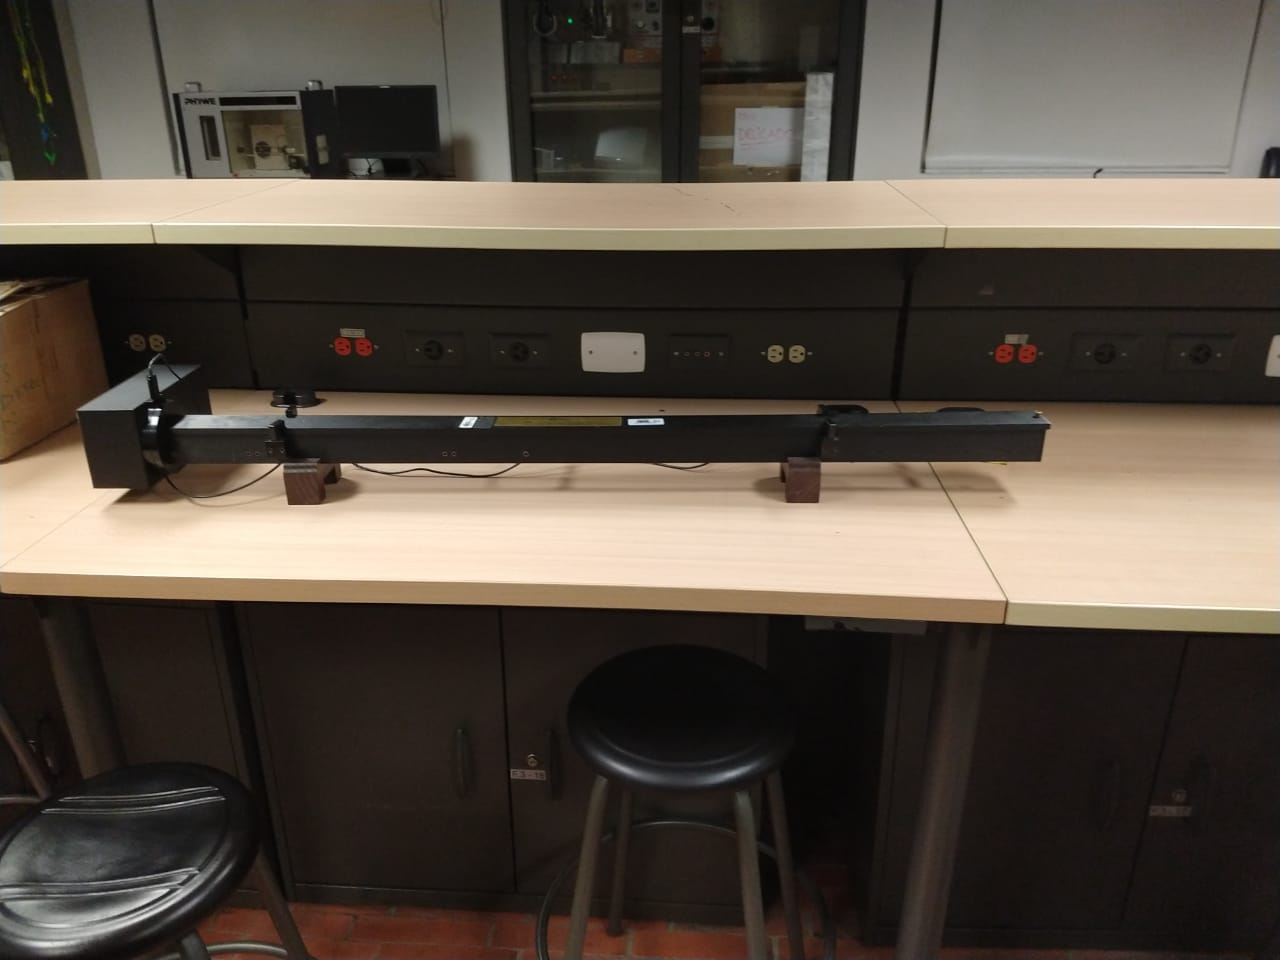
\includegraphics[scale=0.1]{Double_Slit/Figuras/MontajeCompleto.jpg}
    \caption{Montaje completo para práctica de doble rendija.}
    \label{montajecompleto}
\end{figure}
 Este montaje está constituido de un láser y una luz blanca dentro del riel de un metro, los cuales pueden ser activados de un equipo a la vez, una rendija sencilla, una doble rendija con una rendija bloqueadora y una rendija detectora. Adicionalmente, este riel posee un foto detector, photon counting module de la compañía Teach Spin, como muestra la figura \ref{fotodetector}. Adicional a esto, también existe un multiplicador, de voltaje para aumentar la el voltaje leído en el multímetro, con un factor de 1/1000 V con referencia al voltaje registrado. Con todos estos equipos y el láser se realizará el primer experimento.
 
\begin{figure}
    \centering
    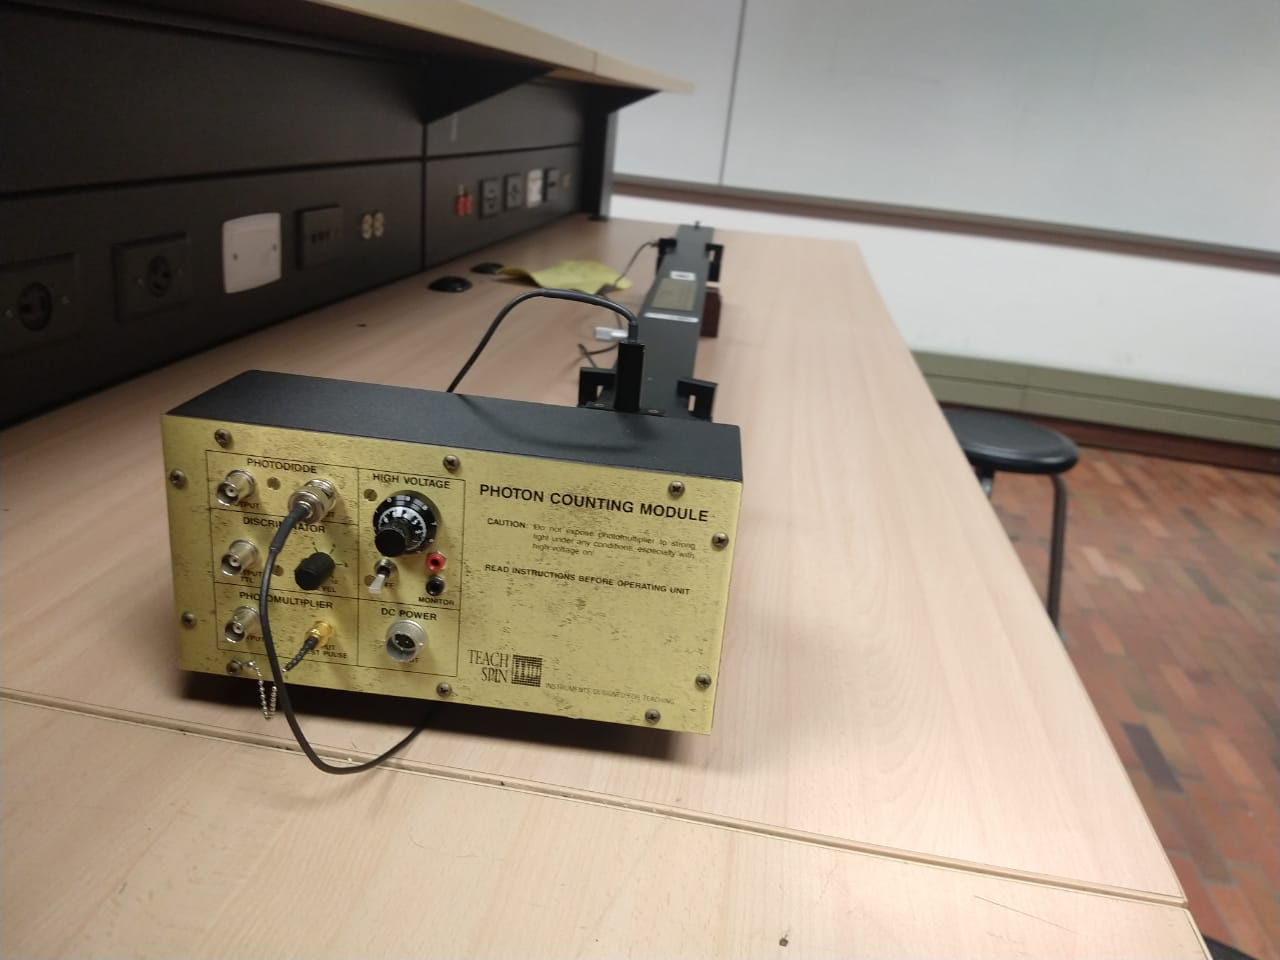
\includegraphics[scale=0.1]{Double_Slit/Figuras/Foto_detector.jpg}
    \caption{Fotodetector con amplificador de voltaje}
    \label{fotodetector}
\end{figure}

Para el segundo experimento, se utiliza el mismo montaje, pero antes se utiliza un osciloscopio, como muestra la figura \ref{osciloscopio}, el cual se usará para calibrar la intensidad de la luz blanca emitida con un filtro de luz verde.

\begin{figure}
    \centering
    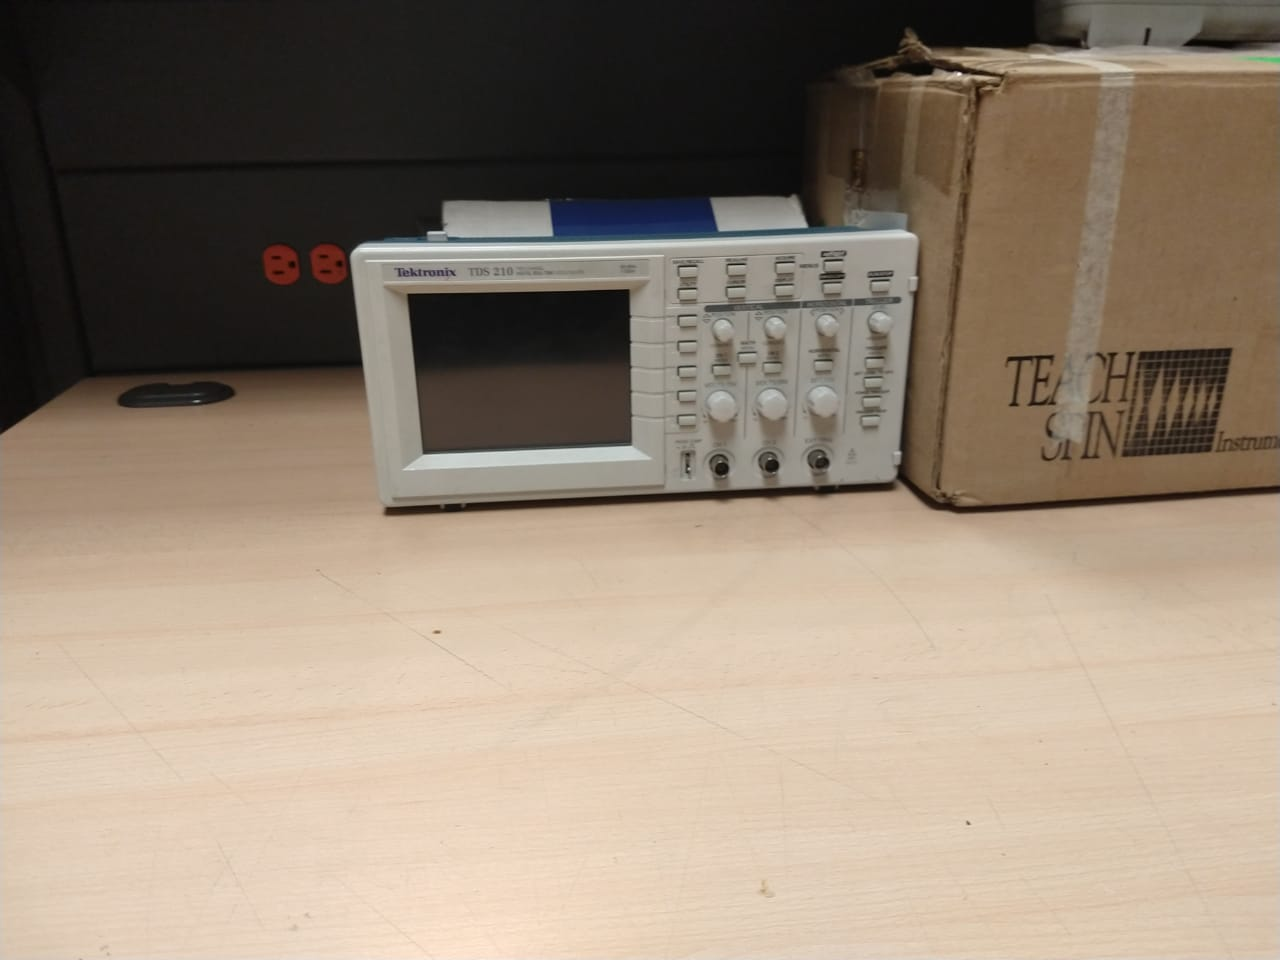
\includegraphics[scale=0.1]{Double_Slit/Figuras/Osciloscopio.jpg}
    \caption{Osciloscopio usado para calibrar la señal de luz blanca que llega al fotomultiplicador}
    \label{osciloscopio}
\end{figure}

Una vez calibrado este haz de luz, se utiliza el contador de frecuencias, Frequency detector de BK precision (figura \ref{contador}, el cual realiza conteo de partículas cada segundo y posee una eficiencia del 4{%}. 

\begin{figure}
    \centering
    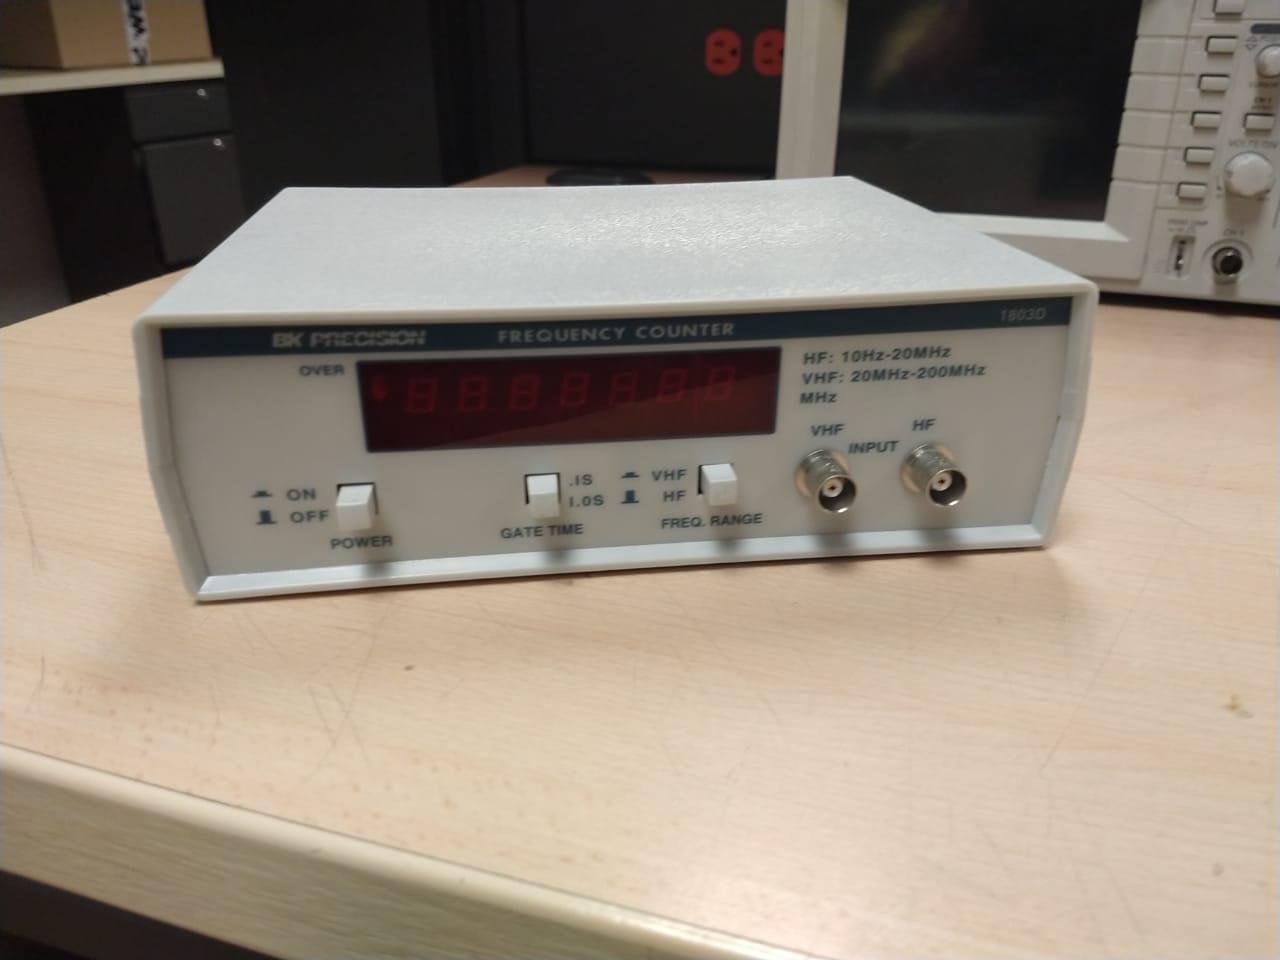
\includegraphics[scale=0.1]{Double_Slit/Figuras/Contador.jpg}
    \caption{Contador BK precision para realizar registrar el número de fotones que ingresan al fotomultiplicador}
    \label{contador}
\end{figure}

%-----------------RESULTADOS----------------------
\section{Resultados y Análisis}
\subsection{Patrón de Interferencia}
Los resultados de las pruebas de las intensidades del láser en el punto del máximo para la doble rendija y las rendijas individuales son mostradas en el cuadro \ref{comparacion_tabla}. A partir de este cuadro, se puede apreciar como la intensidad dada por la doble rendija simplemente no es la suma de ambas de las intensidades de cada una de las rendijas, esto es una evidencia clara de que la ecuación \eqref{difrac} explica por que en el fenómeno de interferencia es necesario incluir un término tal que la intensidad total es mayor que la suma de cada intensidad.


\begin{table}[h]
\begin{tabular}{c|c}
\textbf{Rendija} & \multicolumn{1}{l}{\textbf{Intensidad $(\pm 0.005)[V]$}} \\ \hline\hline
\textbf{Doble} & $1.11$ \\
\textbf{Izquierda} & $0.21$ \\
\textbf{Derecha} & $0.24$
\end{tabular}
\caption{Test cualitativo de los máximos para una doble rendija.}
\label{comparacion_tabla}
\end{table}

Para cada una de estas configuraciones, sus patrones de interferencia fueron medidos. Los resultados se muestran en las figuras \ref{patron_de_una} y \ref{patron_de_dos} se muestran los resultados obtenidos junto a sus respectivos ajustes.

\begin{figure}[ht]
\center{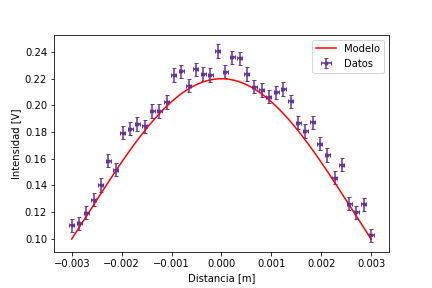
\includegraphics[width=0.39\textwidth,trim={1.5cm 0.5cm 1.5cm 0.5cm}]
{../Figuras/Intensidad_una_rojo.png}}
\caption{\label{patron_de_una}Patrón de interferencia de una sola rendija. Los puntos en morado representan los datos obtenidos experimentalmente y la curva en rojo corresponde a un ajuste efectuado con $\lambda=669nm$.}
\end{figure}

\begin{figure}[h]
\center{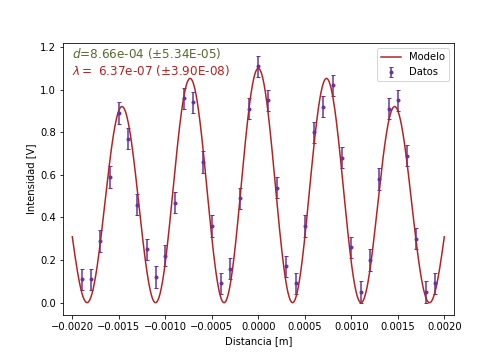
\includegraphics[width=0.39\textwidth,trim={1.5cm 0.5cm 1.5cm 0.5cm}]
{../Figuras/Interferencia_laserrojo.png}}
\caption{\label{patron_de_dos}Patrón de interferencia de doble rendija. Los puntos en morado representan los datos obtenidos experimentalmente y la curva en rojo corresponde a un ajuste efectuado con $\lambda=637nm$ y una distancia entre rendijas de $d=0.866mm$.}
\end{figure}
 Con el fin de ajustar lo parámetros que mejor se ajustan a los datos obtenidos se obtuvo un valor de longitud de onda de  $\lambda=669(\pm 5) nm$ y $\lambda=637(\pm 4) nm$ respectivamente. El resultado obtenido para la doble rendija difiere significativamente de las especificaciones proporcionadas por el láser, no obstante el resultado sigue estando dentro del rango del rojo, se tiene que el origen de esta predicción surge a partir del algoritmo necesario al ajustar tanto la longitud de onda la separación entre los centros de las rendijas.
\subsection{Medición con un fotón a la vez}
Dado que esta parte de la práctica se efectuó haciendo uso de un foto multiplicador, se tuvo como objetivo principal el caracterizar como dependía el conteo de fotones en función del voltaje aplicado. En la figura \ref{fotomultiplicador} se muestra el comportamiento del contador en función del voltaje aplicado.

\begin{figure}[ht]
\center{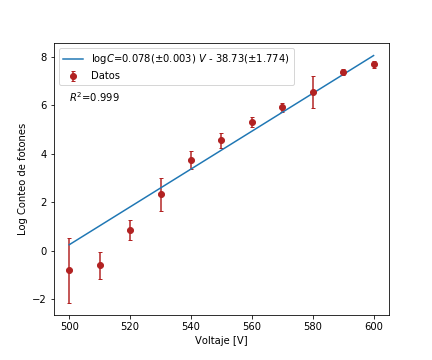
\includegraphics[width=0.35\textwidth,trim={1.5cm 1cm 1.5cm 0.5cm}]
{../Figuras/fotomultiplicador.png}}
\caption{\label{fotomultiplicador}Comportamiento de los conteos (TTL) en función del voltaje en el foto multiplicador. Los puntos en rojo corresponden a los datos obtenidos y la curva azul corresponde al ajuste efectuado.}
\end{figure}

De la figura \ref{fotomultiplicador} se tiene que el conteo de los fotones cumple entonces una ley exponencial en función del voltaje aplicado, el cual cumple con un ajuste de la forma:
\begin{equation}
C=1.51\times10^{-17}\cdot e^{0.078V}.
\end{equation}

\begin{figure}[h]
\center{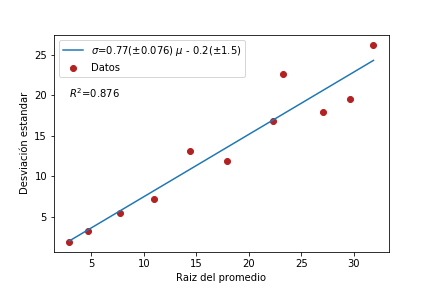
\includegraphics[width=0.35\textwidth,trim={1.5cm 0.5cm 1.5cm 0.5cm}]
{../Figuras/sqrt_promedio_std.png}}
\caption{\label{promedios_std} Gráfico de la raíz del promedio de conteos a una intensidad dada, los puntos en rojo corresponden a los datos experimentales y la linea azul corresponde al ajuste efectuado.}
\end{figure}

Seguido a esto se vario la intensidad del láser a un voltaje de $530 V$ y se observó el comportamiento de la raíz del promedio en función de la desviación estándar, esto con el fin de probar si efectivamente se obtiene un comportamiento de tipo lineal como se espera\footnote{Se espera que la distribución de los conteos se asemeje a una distribución de Poisson dado que la luz que está entrando en el sensor es coherente.}. En la figura \ref{promedios_std} se muestran los resultados obtenidos para este comportamiento. Aunque no se obtuvo lo esperado ($\sigma=\sqrt{\mu}$), si se tiene una relación similar ($\sigma=0.77\sqrt{\mu}$).


Con el fin de ilustrar esto, se efectuó un ``KDE''\footnote{Kernel Density Estimation} con el método de ``Silverman'' y se comparó con la distribución de Poisson con parámetro $k=\langle n\rangle=23$. Para comparar que tan similar eran estas dos se calculó la divergencia de Kullback-Leibler y se obtuvo un valor de $D_{KL}=0.014$, lo cual indica que ambas distribuciones parecen asemejarse bastante.

\begin{figure}[h]
\center{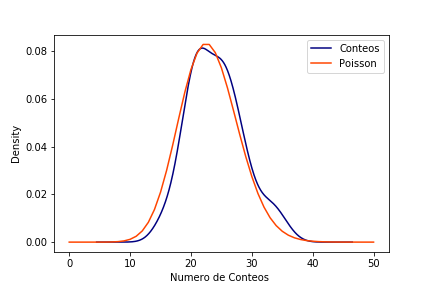
\includegraphics[width=0.35\textwidth,trim={1.5cm 0.5cm 1.5cm 0.5cm}]
{../Figuras/Distribucion.png}}
\caption{\label{distribucion} Distribucion de probabilidad en función del numero de conteos del sensor, la linea narajana corresponde a una distribución de Poisson con parámetro $\langle n\rangle$ y la curva azul corresponde al estimado dado por los datos.}
\end{figure}
Una vez caracterizado el comportamiento del sensor y el conteo de fotones se midió el patrón de interferencia A continuación en la figura \ref{interferencia_laserverde} se muestran los datos experimentales obtenidos al fijar el voltaje del foto multiplicador en $530\ V$ y su intensidad en el valor máximo.
\begin{figure}[h]
\center{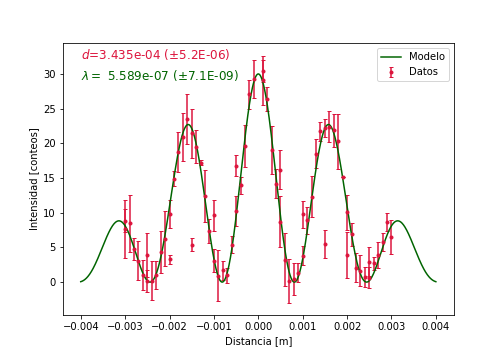
\includegraphics[width=0.35\textwidth,trim={1.5cm 1cm 1.5cm 0.5cm}]
{../Figuras/Interferencia_verde.png}}
\caption{\label{interferencia_laserverde} Gráfica del patrón de interferencia junto a su ajuste respectivo, los parámetros obtenidos a partir del ajuste fueron $\lambda\approx 558 nm$, la longitud de onda de la fuente y $d\approx 0.343 mm$, la distancia entre las rendijas.}
\end{figure}


Como se puede apreciar en la figura \ref{interferencia_laserverde} para el caso de la bombilla con el filtro verde también exhibe el mismo patrón de interferencia en la intensidad que el láser, sin embargo, esta curva tiende a ser menos suave que la del láser, esto se debe principalmente a que al hacer uso de un foto multiplicador, la precisión del instrumento se reduce significativamente, no obstante, se tiene que la intensidad aumenta, con lo cual se logra observar el patrón de interferencia. De acuerdo al ajuste se tiene que la longitud de onda de la fuente es de $\lambda=558(\pm 7)\ nm$ y la distancia entre los centros de las rendijas es de $d=0.343(\pm 5) mm$. Ambos valores parecen tener coherencia con lo reportado en la guía y con el hecho de que la fuente fuera de color verde \footnote{Con el filtro verde, según la referencia \cite{guia} del aparato se tiene un rango de longitud de ondas entre los $541nm$ y los  $551 nm$)}.\\
Dado que el sensor que se utilizó tenía una eficiencia del $5\%$ de detección en el rango de longitud de onda del verde, se calculó la cantidad de fotones incidentes y con esto se estimó el tiempo de un pulso, los resultados se muestran en el cuadro \ref{tiempos_de_viaje}.

\begin{table}[h]
\begin{tabular}{|c|c|c|}
\hline
\textbf{\begin{tabular}[c]{@{}c@{}}Fotones\\  Incidentes\end{tabular}} & \textbf{\begin{tabular}[c]{@{}c@{}}Periodo de\\  un pulso\end{tabular}} & \textbf{\begin{tabular}[c]{@{}c@{}}Tiempo de viaje \\ de $1m$\end{tabular}} \\ \hline
$620$                                                                  & $1.612\times 10^{-4} s$                                                   & $3.34\times 10^{-9} s$                                                        \\ \hline
\end{tabular}
\caption{Tiempos que toman los pulsos en llegar a través del camino hasta el detector}
\label{tiempos_de_viaje}
\end{table}
 Esto lo que nos muestra es que la configuración utilizada en el montaje experimental fue tal que se podía garantizar que tan sólo un fotón está pasando por la rendija. Esto tiene como resultado principal que aún teniendo la condición de un solo fotón pasando a la vez por la rendija, el comportamiento de tipo onda sigue siendo apreciado como se muestra en la figura \ref{interferencia_laserverde}. Con esto se concluye que los fotones no sólo interfieren con otros fotones si no que también lo hacen consigo mismos, siendo esto la dualidad onda-partícula.

%---------------CONCLUSIONES-------------------

\section{Conclusiones}
\begin{itemize}
    \item Al observar el montaje experimental realizado y las figuras \ref{difraccion} y \ref{interferencia_laserverde}, se logró realizar el experimento de Young y visualizar los patrones de interferencia. Al observar la figura \ref{difraccion}, pudimos ver el patrón de interferencia para la una rendija simple, y con la figura \ref{interferencia_laserverde} observamos el patrón de interferencia para la doble rendija, tanto para un láser como para un haz de luz blanca con filtro. Para la doble rendija se observa un comportamiento similar en ambos tipos de luz, sin embargo, la luz con filtro se ve menos suavizada dada la presencia del foto multiplicador.
    \item Al medir la interferencia con el fotodiodo y el fotomultiplicador se puede comprobar, usando el láser, como la intensidad de la doble rendija es cercana a cuatro veces mayor, al mirar la suma de suma las rendijas ubicadas a izquierda y derecha y comparar con la doble rendija en \ref{comparacion_tabla}. Las discrepancia de estos datos (23{\%}), puede ser atribuida al rango de distancias dónde estaban ubicados los máximos de cada rendija. Al comparar esto, con los cálculos analíticos de la sección dos, se comprueba la naturaleza ondulatoria de la luz, pues los datos experimentales dan soporte a estos. 
    \item Con el segundo experimento, usando el detector de partículas y al comparar los tiempos de viaje de y detección, fue posible observar el comportamiento corpuscular de la luz, dado que el tiempo de viaje fue mucho menor (5 órdenes de magnitud), hay una garantía de que en efecto, el número de fotones que pasó por la rendija no fue uno, pues el comportamiento mostrado en la figura \ref{interferencia_laserverde}, es el esperado.
    \item La comparar los resultados encontrados para los datos medidos y observar las difracciones esperadas de Fraunhofer y Fresnel, se observa que los patrones son muy similares, por lo que mientras se tengan distancias cortas (aproximadamente un metro) ambas teorías concuerdan.
\end{itemize}
%Se deben contestar las preguntas planteadas inicialmente o dar las razones por las cuales no es posible hacerlo. Las conclusiones deben ser necesariamente una consecuencia del experimento realizado, es decir que no se deben tocar aspectos que no se hayan expuesto en la sección de resultados y análisis. Si escribe algo que no se encuentra en la sección de resultados y análisis, esto quiere decir que hace falta incluir material en resultados y análisis. Concluir únicamente aspectos pertinentes a su trabajo en el laboratorio; evite generalizaciones que no hablan concretamente de lo que usted hizo o midió.

\begin{thebibliography}{9}
\bibitem{opticaondulatoria}
Université Moulay Ismaïl, 2017
\url{https://www.overleaf.com/project/5c58b017b206d66446cbc4bd}
\bibitem{MIT} 
Massachusetts Institute of Technology
\url{http://web.mit.edu/viz/EM/visualizations/coursenotes/modules/guide14.pdf}
\bibitem{guia} 
Inc. David A. Van Baak; TeachSpin. Two-slit interference one photon at a time \textit{The Essential Quantum Paradox}, instruction manual
Suite 409 Buffalo NY, 2013.
\url{http://physics-astronomy-manuals.wwu.edu/TeachSpin\%20Two\%20Slit\%20Expanded\%20Manual.pdf}
\end{thebibliography}

\end{document}
%
% ****** End of file apssamp.tex ******
